\chapter{Implementación}
En este séptimo capítulo se detallará la implementación del sistema. En primer lugar,  se presentará la estructura del proyecto que se ha realizado para el frontend y del backend y, a continuación,
se describirá la implementación de cada una de las funcionalidades del sistema, presentando la documentación de cada ruta de la API y describiendo el código escrito durante el desarrollo.

\section{Herramientas utilizadas}
En el desarrollo de la aplicación se utilizarán varias herramientas externas que ayudarán en el cumplimiento de los objetivos y facilitarán la implementación de cada una de las historias de usuario. A continuación se muestran algunas
de ellas:

\subsection{Git \& Github}
Git es una herramienta para el control de versiones. Nos permitirá mantener un historial de cambios que nos ayudarán en la implementación cuando necesitemos "volver atrás", así como poder trabajar en distintas ramas cuando la situación lo requiera (por ejemplo, si encuentro un error puedo abrir una nueva rama para poder trabajar exclusivamente en arreglarlo).

Como complemento a Git, usaremos Github, una plataforma para alojar repositorios de Git. En Github tendremos un repositorio para el frontend y para el backend, donde se irán subiendo los cambios que se vayan realizando. Esto facilitará la posibilidad de trabajar en el desarrollo en varios dispositivos permitiendo un desarrollo más flexible a la hora de dónde (en qué dispositivo) y cuándo trabajar. 

\subsection{Jira}
Jira es una herramienta para la gestión de proyectos. Usaré Jira para facilitar el cumplimiento de algunos de los principios de metodologías ágiles que usamos en la planificación y controlar el seguimiento de esta última. En Jira tendré un Sprint Backlog, cuyas historias de usuario y tareas irán moviéndose a los distintos Sprints para su desarrollo.

\begin{figure}[H]
  \centering
  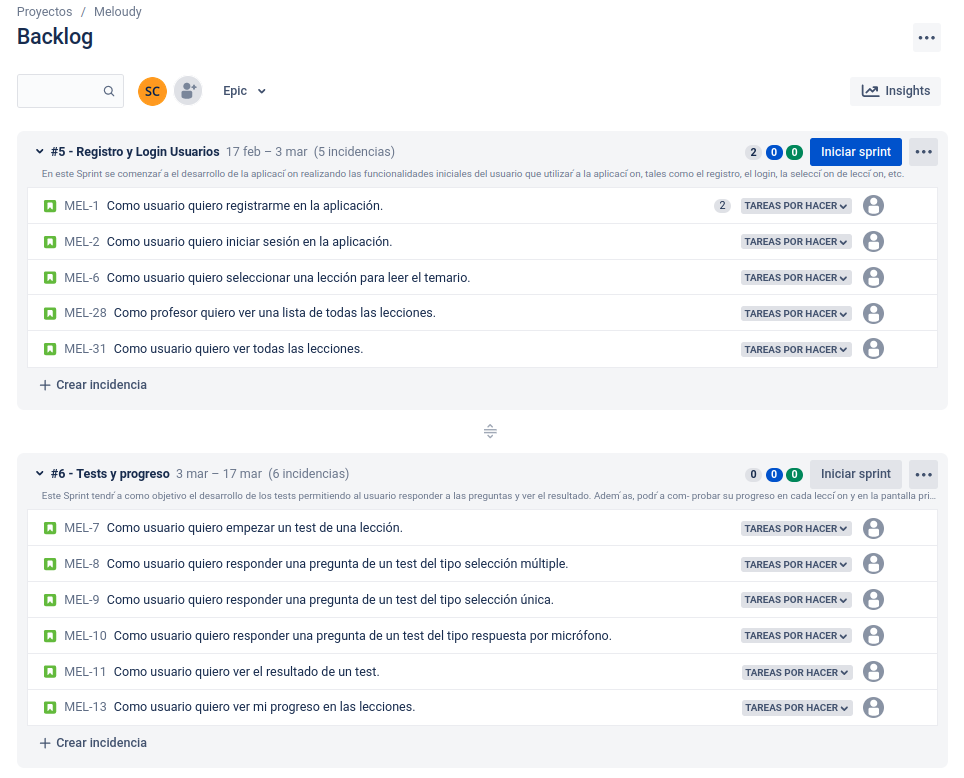
\includegraphics[width=\textwidth]{imagenes/c7/jira.png}
  \caption{Captura de pantalla de Jira. En ella se puede ver el Sprint Backlog, donde se encuentran las historias de usuario repartidas entre los sprints.}
  \label{fig:login}
\end{figure}


\subsection{Visual Studio Code \& Android Studio}
Visual Studio Code es el editor de código fuente que se usará para implementar la parte backend (NodeJS) de nuestro sistema. Nos permitirá un desarrollo más cómodo y eficiente, ya que nos ofrece una gran variedad de herramientas para el desarrollo de código, como la posibilidad de depurar el código, herramientas para el formato del código, visualizador de versiones de Git, etc.

Android Studio es el entorno de desarrollo integrado oficial para la plataforma Android. Se utilizará para implementar la parte de frontend (flutter) y para ejecutar la aplicación en un simulador de Android o en nuestro propio dispositivo físico.

\subsection{Mongo Compass}
Mongo Compass es una herramienta interactiva para la consulta, la gestión y el análisis de los datos en MongoDB. Se utilizará para comprobar si las consultas se realizan correctamente y para añadir datos a la base de datos (lecciones, preguntas...) de forma fácil, cómoda y rápida.

\begin{figure}[H]
  \centering
  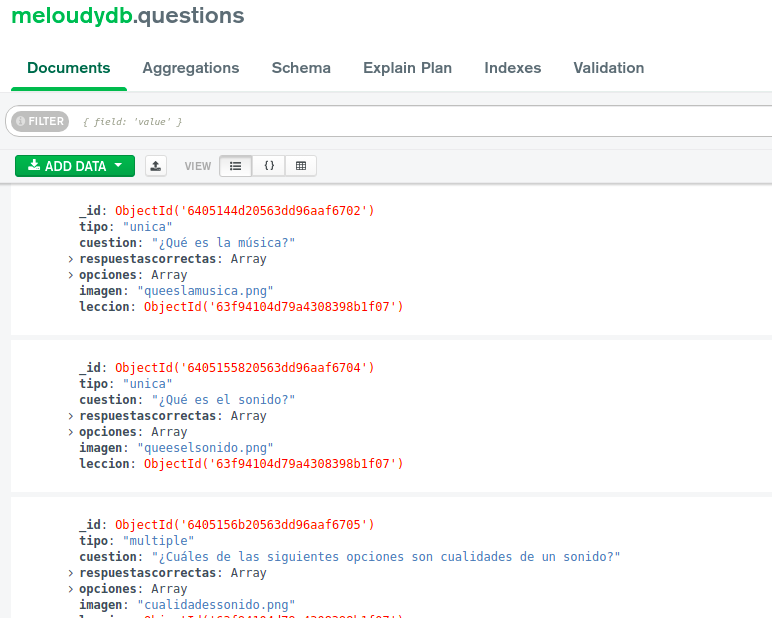
\includegraphics[width=\textwidth]{imagenes/c7/compass.png}
  \caption{Captura de pantalla de Jira. En ella se puede ver el Sprint Backlog, donde se encuentran las historias de usuario repartidas entre los sprints.}
  \label{fig:login}
\end{figure}

\subsection{Postman}
Postman es una plataforma API para diseñar, construir, probar e iterar APIs. Se utilizará en la implementación de nuestra aplicación para comprobar el funcionamiento de las rutas especificadas y codificadas en el backend. Además podremos realizar una documentación de nuestra API mediante
esta herramienta para facilitar la comprensión y el mantenimiento de cada ruta.



\section{Estructura del proyecto}
\label{sec:estructura}
Como se mencionó en la arquitectura del sistema en el anterior capítulo, el proyecto se ha desarrollado en dos partes, una parte de frontend y otra de backend. La parte de frontend se ha desarrollado en Flutter y la parte de backend se ha desarrollado en Node.js. 

La estructura del proyecto se puede ver en la siguiente imagen:
\begin{figure}[H]
  \centering
  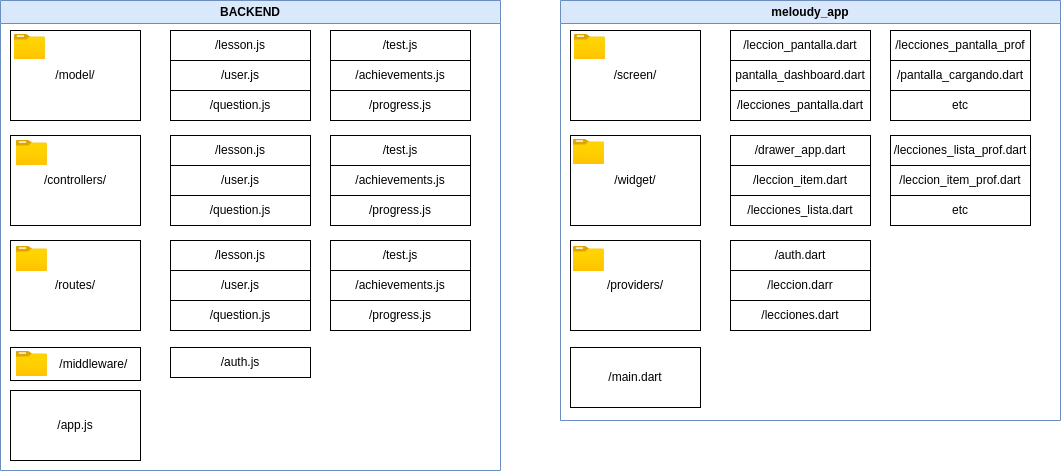
\includegraphics[width=\textwidth]{imagenes/c7/estructura.png}
  \caption{Estructura del proyecto, donde se puede ver la parte de frontend y la parte de backend.}
  \label{fig:login}
\end{figure}

En la figura anterior podemos ver que el desarrollo del proyecto se ha realizado en dos partes, una parte de frontend y otra de backend.

La parte de backend se ha desarrollado en Node.js, por lo que se han dividido los archivos en carpetas de acuerdo a su funcionalidad:
\begin{itemize}
    \item \textit{app.js}: Archivo principal de la aplicación. En él se configura el servidor y se importan las rutas.
    \item \textit{routes}: Carpeta que contiene las rutas de la API. Dentro se encuentran distintos archivos que contienen las rutas de cada entidad de la base de datos (user, lesson, question...).
    \item \textit{controllers}: Carpeta que contiene los controladores de las rutas de la API. Dentro se encuentran distintos archivos que contienen los controladores de cada entidad de la base de datos (user, lesson, question...)
    \item \textit{models}: Carpeta que contiene los modelos de la base de datos.
    \item \textit{middleware}: Carpeta que contiene los middleware de la aplicación. Por dichos middleware pasarán algunas peticiones que se hagan a la API.
\end{itemize}

La parte de frontend se ha desarrollado en Flutter, por lo que se han dividido los archivos en carpetas de acuerdo a su funcionalidad, dentro de la carpeta \textit{lib}:

\begin{itemize}
  \item \textit{main.dart}: Archivo principal de la aplicación. En él se configura la aplicación y se importan las rutas.
  \item \textit{providers}: Carpeta que contiene los providers de la aplicación. Los providers son clases que se encargan de gestionar el estado de la aplicación.
  \item \textit{screen}: Carpeta que contiene las pantallas de la aplicación. Dentro se encuentran distintos archivos que contiene cada pantalla de la aplicación.
  \item \textit{widgets}: Carpeta que contiene los widgets de la aplicación. Dentro se encuentran los archivos de los widgets que se utilizan en las distintas pantallas de la aplicación.
\end{itemize}

\section{Definición de la API (Backend)}
\label{sec:api}
En esta sección se describirá la API que se ha desarrollado para el sistema. La API se ha desarrollado en Node.js y se ha utilizado el framework Express para trabajar con el protocolo HTTP.

\subsection{Rutas}

\subsubsection{Usuarios}
\label{sec:usuarios}
La API cuenta con las siguientes rutas para la gestión de usuarios:

\begin{itemize}
    \item \textit{POST /api/user/registro}: Ruta para registrar un usuario. Recibe los datos del usuario en el cuerpo de la petición, encripta la contraseña y almacena todos los datos en la base de datos. Si el usuario se registra correctamente, se devuelve un token que se utilizará para la autenticación de las peticiones que se hagan a la API.
    \item \textit{POST /api/user/login}: Ruta para iniciar sesión. Recibe los datos del usuario en el cuerpo de la petición y comprueba si el usuario existe en la base de datos. Si el usuario existe, se comprueba que la contraseña sea correcta. Si la contraseña es correcta, se devuelve un token que se utilizará para la autenticación de las peticiones que se hagan a la API.
    \item \textit{GET /api/user/get-user/\{id\}}: Ruta para obtener los datos de un usuario. Recibe por parámetro el id del usuario y devuelve los datos de dicho usuario.
    \item \textit{GET /api/user/get-users}: Ruta para obtener los datos de todos los usuarios. No recibe ningún parámetro y devuelve una lista de los datos de todos los usuarios.
%    \item \textit{PUT /api/user}: Ruta para actualizar los datos de un usuario. Recibe los datos del usuario en el cuerpo de la petición y los actualiza en la base de datos. Si el usuario se actualiza correctamente, se devuelve un token que se utilizará para la autenticación de las peticiones que se hagan a la API.
    \item \textit{DELETE /api/user/delete-user/\{id\}}: Ruta para eliminar un usuario. Recibe por parámetro el id del usuario y lo elimina de la base de datos.
    
\end{itemize}

\subsubsection{Lecciones}
\label{sec:lecciones}
La API cuenta con las siguientes rutas para la gestión de lecciones:

\begin{itemize}
%    \item \textit{POST /api/lesson/get-lessons/\{id\}}: Ruta para crear una lección. Recibe los datos de la lección en el cuerpo de la petición y los almacena en la base de datos. Si la lección se crea correctamente, se devuelve la lección creada.
%    \item \textit{GET /api/lessons}: Ruta para obtener las lecciones de un usuario. Recibe el token del usuario en el encabezado de la petición y comprueba si el token es correcto. Si el token es correcto, se devuelve las lecciones del usuario.
    \item \textit{POST /api/lesson/get-lessons/\{id\}}: Ruta para obtener los datos de una lección. Recibe por parámetro el id de la lección y se devuelven los datos de esta.
%    \item \textit{PUT /api/lessons/:id}: Ruta para actualizar los datos de una lección. Recibe los datos de la lección en el cuerpo de la petición y los actualiza en la base de datos. Si la lección se actualiza correctamente, se devuelve la lección actualizada.
%    \item \textit{DELETE /api/lessons/:id}: Ruta para eliminar una lección. Recibe el token del usuario en el encabezado de la petición y comprueba si el token es correcto. Si el token es correcto, se elimina la lección de la base de datos.
  \end{itemize}

\subsubsection{Preguntas}
\label{sec:preguntas}
La API cuenta con las siguientes rutas para la gestión de preguntas:

\begin{itemize}
  \item \textit{GET /api/question/get-questions}: Ruta para obtener todas las preguntas almacenadas en la base de datos.
  \item \textit{GET /api/question/get-questions/\{idLeccion\}}: Ruta para obtener las preguntas de una lección. Recibe por parámetro el id de la lección y devuelve todas las preguntas existentes de dicha lección.
  \item \textit{GET /api/question/get-question-test/\{idTest\}}: Ruta para obtener las preguntas de un test. Recibe por parámetro el id del test y devuelve todas las preguntas existentes de dicho test junto con el propio test.
  \item \textit{GET /api/question/get-question/\{id\}}: Ruta para obtener los datos de una pregunta. Recibe por parámetro el id de la pregunta y devuelve los datos de dicha pregunta.
\end{itemize}

\subsubsection{Tests}
\label{sec:tests}
La API cuenta con las siguientes rutas para la gestión de tests:

\begin{itemize}
  \item \textit{GET /api/progress/get-tests-progress/\{idUsuario\}/\{idLeccion\}}: Ruta para obtener todos los tests de un usuario en una lección. Recibe por parámetro el id del usuario y el de la lección, busca el progreso a partir de estos identificadores, busca todos los tests de dicho progreso y los devuelve.
\end{itemize}


\subsubsection{Progress}
\label{sec:progress}
La API cuenta con las siguientes rutas para la gestión del progreso de los usuarios:

\begin{itemize}
  \item \textit{POST /api/progress/create-test-and-progress/}: Ruta para crear un test y el progreso de un usuario. Recibe los datos del test y del progreso en el cuerpo de la petición y los almacena en la base de datos. Si el progreso ya estaba creado, solamente se almacena el nuevo test y se añade a la lista de tests del progreso. Si el test y el progreso se crean correctamente, se devuelve el test y el progreso creados. 
\end{itemize}




\subsection{Middleware}
\label{sec:middleware}
Un middleware es una función que se ejecuta antes de que se ejecute otra. Se utiliza para realizar acciones comunes a varias funcionalidades. La API cuenta con los siguientes middleware:

\begin{itemize}
  \item \textit{auth}: Middleware que comprueba si el token del usuario es correcto (es decir, si el usuario está identificado en la aplicación). Si el token es correcto, se pasa a la siguiente función. Si el token no es correcto, se devuelve un error.
%  \item \textit{authAdmin}: Middleware que comprueba si el token del usuario es correcto y si el usuario es administrador. Si el token es correcto y el usuario es administrador, se pasa a la siguiente función. Si el token no es correcto o el usuario no es administrador, se devuelve un error.
\end {itemize}

\newpage
\section{Funcionalidad de inicio}
\label{sec:inicio}
A continuación presentamos la funcionalidad básica de la aplicación que usará cualquier usuario que se registre:


% \subsection{Pantallas y Widgets básicos}
% \label{sec:widgets}
% La aplicación cuenta con una serie de pantallas y widgets que se utilizan en todas las pantallas de la aplicación. 
% Estos widgets se han desarrollado para que se puedan reutilizar en las distintas pantallas de la aplicación. A continuación se describen los widgets y pantallas que se han desarrollado:


\subsection{Drawer}
Un drawer es un menú lateral que se puede abrir y cerrar y que se utiliza para acceder a distintas pantallas de la aplicación. En este caso, se
abre y se cierra clickando en el icono superior izquierdo de la aplicación. Se ha utilizado el llamado "menú hamburguesa". En la siguiente imagen se puede ver el drawer abierto:

\begin{figure}[H]
    \centering
    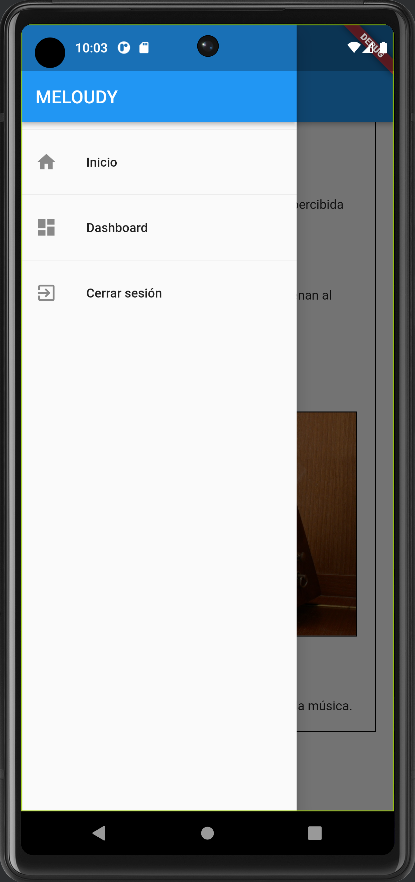
\includegraphics[width=0.4\textwidth]{imagenes/c7/drawer.png}
    \caption{Drawer abierto en la aplicación con tres opciones (por ser desde la vista del profesor): Inicio, Dashboard y Cerrar sesión.}
    \label{fig:drawer}
\end{figure}


\subsection{Sesión}
\label{sec:sesion}
Se han desarrollado tres características adicionales relacionadas con la sesión de usuario y que explicaremos con más detalle en cada uno de los apartados de la sesión.
\begin{itemize}
    \item \textbf{Encriptación de la contraseña:} La contraseña del usuario se encripta antes de ser almacenada en la base de datos para evitar que sea visible por cualquier persona que tenga acceso a esta. De esta forma
    garantizamos que se cumple el requisito de seguridad de la contraseña. Para esto se ha utilizado un algoritmo hash de la librería \textit{bcrypt}.
    El diagrama que explica el proceso de encriptación se muestra en la siguiente imagen:
    \begin{figure}[H]
      \centering
      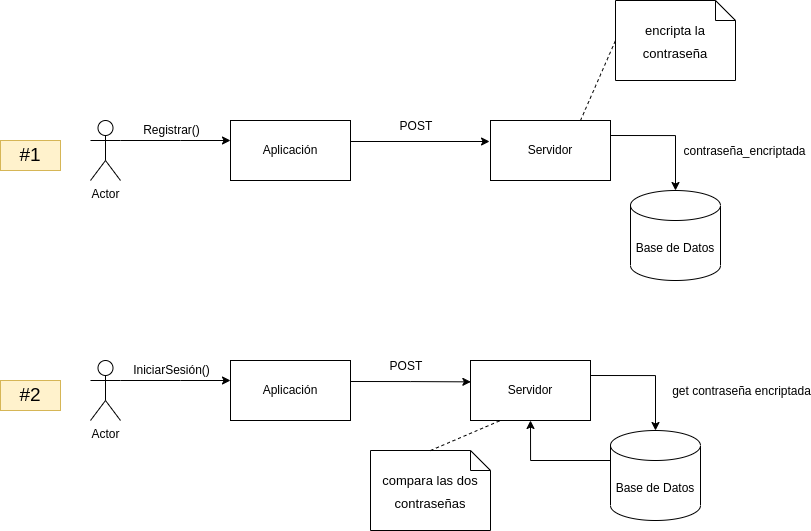
\includegraphics[width=0.9\textwidth]{imagenes/c7/logindiag.png}
      \caption{Diagrama que explica el proceso de encriptación en el inicio de sesión desarrollado en la aplicación.}
      \label{fig:login}
    \end{figure}

    \item \textbf{Intercambio de token:} El servidor proporciona un token al usuario cuando se registra o inicia sesión. Este token se añade a las peticiones que se hagan a la API. De esta forma, garantizamos que se cumple el requisito de seguridad de la sesión y 
    que todas las peticiones válidas que se hagan a la API son de usuarios registrados. Además, el token fija una fecha de expiración al crearse para aumentar la seguridad del usuario. Esta funcionalidad se ha logrado con el paquete \textit{jsonwebtoken} de NodeJS.
    El diagrama que explica el proceso de intercambio de token se muestra en la siguiente imagen:

    \begin{figure}[H]
      \centering
      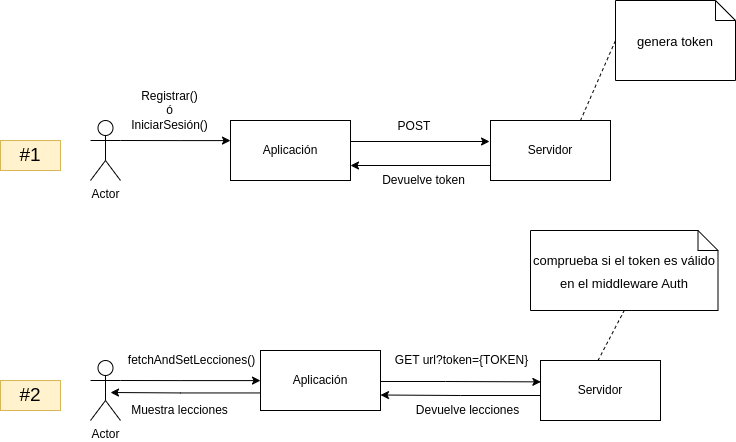
\includegraphics[width=0.9\textwidth]{imagenes/c7/tokendiag.png}
      \caption{Diagrama que explica el proceso de intercambio de token en el inicio de sesión desarrollado en la aplicación.}
      \label{fig:token}
    \end{figure}

    \item \textbf{Sesión entre instancias:} La sesión se mantiene entre instancias de la aplicación. Es decir, si el usuario cierra la aplicación y la vuelve a abrir, no tendrá que volver a iniciar sesión si no ha cerrado la sesión o si el token no ha expirado. 
    Esto se ha conseguido mediante el almacenamiento del token en la memoria local del dispositivo con la librería \textit{shared\_preferences}. De esta forma, cuando el usuario inicia sesión, el token se almacena en el almacenamiento local del dispositivo 
    y cuando el usuario cierra la aplicación y la vuelve a abrir, el token se recupera del almacenamiento local del dispositivo y se comprueba si es correcto. Si es correcto, se pasa a la siguiente pantalla. Si no es correcto, se vuelve a la pantalla de inicio de sesión.
    Este token además estará siendo comprobado constantemente para que si el este expira, se cierre la sesión y se vuelva a la pantalla de inicio de sesión evitando accesos no autorizados.

    El diagrama que explica el proceso de sesión entre instancias se muestra en la siguiente imagen:

    \begin{figure}[H]
      \centering
      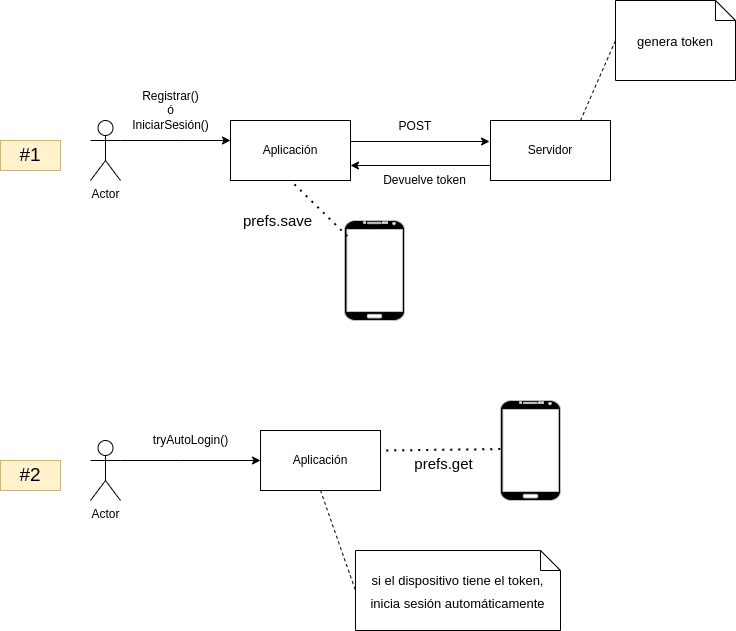
\includegraphics[width=0.9\textwidth]{imagenes/c7/token2.png}
      \caption{Diagrama que explica el proceso de sesión entre instancias en el inicio de sesión desarrollado en la aplicación.}
      \label{fig:sesion}

    \end{figure}

  \end{itemize}

\subsubsection{Inicio de sesión}
\textit{Desarrollado en el Sprint 5}
\label{sec:login}

La aplicación cuenta con una pantalla de inicio de sesión para que los usuarios puedan acceder a la aplicación con su cuenta registrada previamente. 
Para el inicio de sesión, el usuario deberá introducir su nombre de usuario y su contraseña. Si el usuario no tiene una cuenta, podrá registrarse pulsando en el botón 'Registrarse'. En la siguiente imagen se puede ver la pantalla de inicio de sesión:

\begin{figure}[H]%
  \centering
  \subfloat[\centering Pantalla de login]{{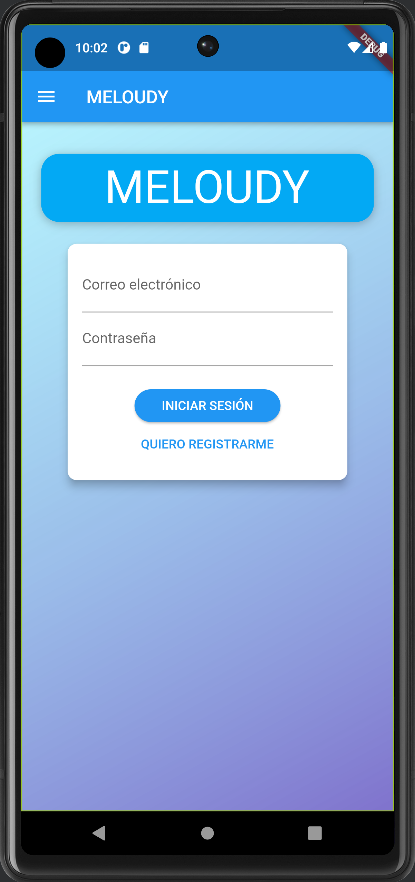
\includegraphics[width=0.40\textwidth]{imagenes/c7/login.png} }}%
  \qquad
  \subfloat[\centering Estructura en componentes de la pantalla de login.]{{ 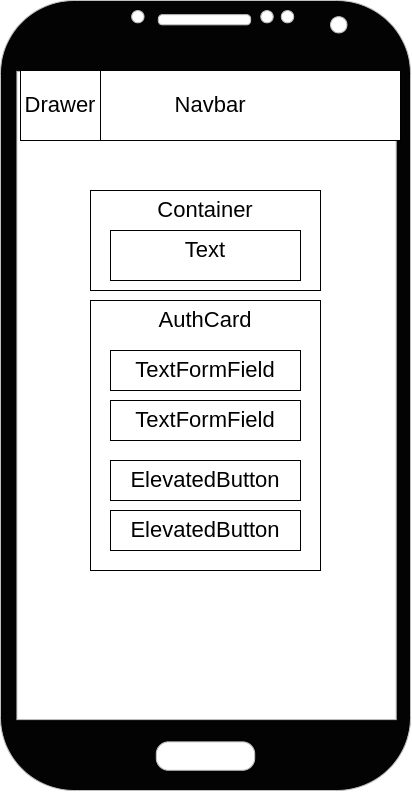
\includegraphics[width=0.45\textwidth]{imagenes/c7/logincompo.png} }}%
  \caption{Pantalla de inicio de sesión del usuario donde se puede ver el formulario de inicio de sesión con los campos de usuario (correo) y contraseña.}%
  \label{fig:login}%
\end{figure}


\paragraph*{Vista}
Empezando por la vista, se ha desarrollado un widget para la pantalla de inicio de sesión. Este widget se compone de un formulario con dos campos de texto, uno para el nombre de usuario y otro para la contraseña. Además, el formulario contiene un botón para iniciar sesión y otro para ir a registrarse si el usuario así lo desea.

La pantalla tiene una pila que contiene dos widgets: un container con un fondo en degradado conseguido con el atributo \textit{gradient} de la clase \textit{BoxDecoration} de Flutter, y un SingleChildScrollView que consta de un widget Column para poder colocar los elementos de forma vertical. Dichos elementos son: un \textit{Container} para el título de la aplicación y un Widget personalizado que contiene el formulario de inicio de sesión \textit{AuthCard()}.
Este último no es más que un widget de la clase \textit{Card} con dos \textit{TextFormField} (uno para el correo electrónico y otro para la contraseña) y un \textit{ElevatedButton} para proceder al inicio de sesión.

\paragraph*{Lógica}
En cuanto a la lógica, una vez el cliente pulsa el botón de 'Iniciar sesión', se llama a la función asíncrona \textit{submit}, la cual se encarga de comprobar que los datos introducidos son correctos.
Cuando los datos son comprobados, se procede a iniciar sesión en la aplicación mediante el método de inicio de sesión del Provider Auth. Para esto, se envia una petición HTTP POST a la ruta \textit{/user/login} de la API con los datos escritos en el formulario de inicio de sesión.

Por otro lado, en el servidor cuando la petición es recibida a dicha ruta, se ejecuta una función en el controlador para el inicio de sesión de usuarios. Esta función capta los valores y comprueba que el usuario existe en la base de datos. Si el usuario existe, se comprueba que la contraseña introducida es correcta mediante el método \textit{verify} de bcrypt. Si los datos son correctos, se genera el token de sesión y se devuelve al cliente. Si el usuario no existe o la contraseña es incorrecta, se devuelve un código de estado 400 y un mensaje de error.

Cuando el cliente recibe la respuesta del servidor, se comprueba si el código de estado es 200, lo que significa que el inicio de sesión ha sido correcto. En este caso, se almacena el token de sesión en el dispositivo tal y como se ha explica en la sección \ref{sec:sesion}. 
\newpage
\subsubsection{Registro}
\textit{Desarrollado en el Sprint 5}
\label{sec:register}

La aplicación cuenta con una pantalla de registro para que los usuarios puedan registrarse en la aplicación. Para el registro, el usuario deberá introducir su nombre de usuario y su contraseña dos veces. Si el usuario ya tiene una cuenta, podrá iniciar sesión pulsando en el botón 'Iniciar sesión'. En la siguiente imagen se puede ver la pantalla de registro:


\begin{figure}[H]
  \centering
  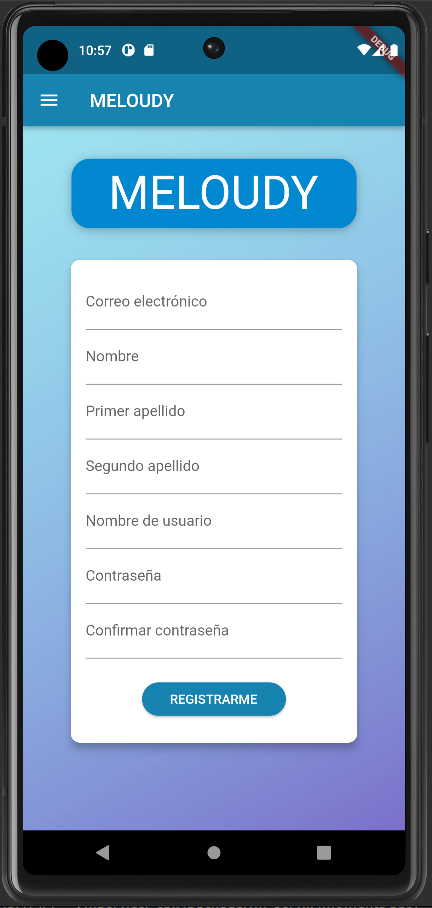
\includegraphics[width=0.4\textwidth]{imagenes/c7/registro.png}
  \caption{Pantalla de registro de los usuarios donde se puede ver el formulario de registro con los campos de usuario (correo), contraseña y repetir la contraseña.}
  \label{fig:register}
\end{figure}

\paragraph*{Vista}
La vista del registro es muy similar a la del inicio de sesión. La única diferencia es que el formulario contiene un campo adicional para introducir la contraseña otra vez por razones de seguridad.


\paragraph*{Lógica}
En cuanto a la lógica, una vez el cliente pulsa el botón de 'Registrarse', también se llama a la función asíncrona \textit{submit}, que se encarga de comprobar que los datos introducidos 
son correctos. Cuando se ha hecho esto, si los datos son válidos, la función llama al método de registro del Provider Auth, el cual envia una petición HTTP POST a la ruta \textit{/user/registro}
 de la API con los datos escritos en el formulario de registro. 

Para poder procesar esta petición de Flutter, una vez el servidor recibe la petición a la ruta de registro, se ejecuta una función en el controlador para el registro de usuarios.
 Esta función capta los valores, encripta la contraseña y crea el usuario en la base de datos. Si los datos son correctos, se genera un token de sesión y
  se devuelve al cliente junto con un código de estado 201 y un mensaje de éxito. Si el registro no es correcto, se devuelve un código de estado 400 y un mensaje de error.

  Cuando Flutter recibe la respuesta del servidor, almacena el token de sesión en el dispositivo tal y como se ha explica en la sección \ref{sec:sesion}.

\subsubsection{Cierre de sesión}
\textit{Desarrollado en el Sprint 5}
\label{sec:logout}

La aplicación cuenta con una opción para cerrar sesión. Para cerrar sesión, el usuario deberá pulsar en el botón \textit{Cerrar sesión} que se encuentra en el drawer (barra lateral) de la aplicación. También se cerrará sesión automáticamente si el token ha expirado.

\paragraph*{Vista}
Para el cierre de sesión, se ha añadido una fila al drawer (barra lateral) de la aplicación, el cual el usuario clicará cuando desee cerrar su sesión.

\paragraph*{Lógica}
La lógica del cierre de sesión es sencilla: se llama a la función \textit{logout} de la clase \textit{Auth} donde se reestablecen los valores de la sesión y se limpian los datos de la sesión almacenados en el dispositivo con el paquete \textit{shared\_preferences}. 
Esta limpieza de datos se realiza en el método \textit{clear}.
Además, se ha añadido un timer que se encarga de cerrar la sesión automáticamente si el token ha expirado. Este timer se ejecuta cada cierto tiempo y comprueba si el token ha expirado. Si es así, se llama al método \textit{logout} mencionado anteriormente.

\newpage

\section{Funcionalidad de usuario}
\label{sec:funcionalidad_usuario}

\subsection{Lista de lecciones}
\textit{Desarrollado en el Sprint 5}

\label{sec:lista_lecciones}
\paragraph*{Vista}
Para que el usuario pueda ver la lista de lecciones, se ha desarrollado un widget principal para la pantalla. Este widget contiene la ListaLecciones, que a su vez estará compuesta de una lista de widgets llamada LeccionItem. Cada uno de estos widgets contendrá la información principal de una lección, como el título y la imagen de perfil. Además, cada uno de estos widgets (LecciónItem) tendrá un botón para acceder a la lección. En la siguiente imagen se puede ver la pantalla de lista de lecciones: : 

\begin{figure}[H]
  \centering
  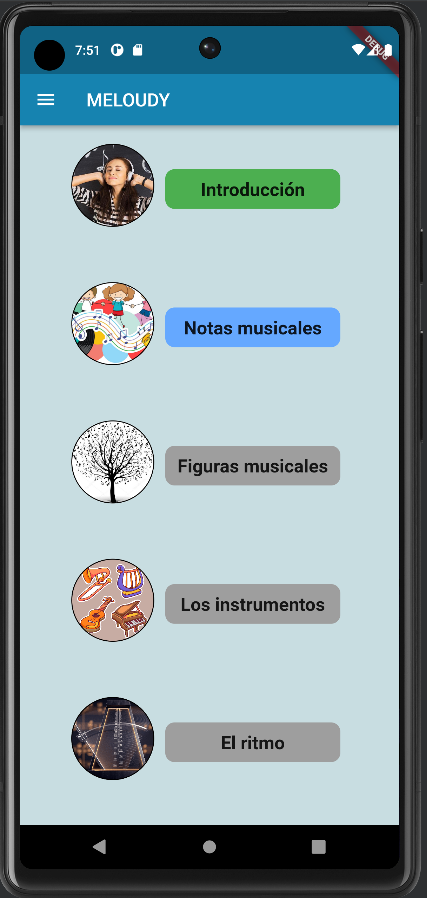
\includegraphics[width=0.4\textwidth]{imagenes/c7/pantprin.png}
  \caption{Pantalla de inicio de sesión}
  \label{fig:login}
\end{figure}

\subsection{Lección} 
\textit{Desarrollado en el Sprint 5}

\label{sec:leccion}
\paragraph*{Vista}
La vista de una lección proporciona al usuario información más detallada de esta. Primero se muestra la imagen de la lección y el título. A continuación, 
se muestra el contenido de la lección en forma de texto, imágenes, vídeos, etc... Esto se ha conseguido construyendo widgets de forma dinámica dependiendo del tipo
de contenido almacenado. Finalmente, se muestra un botón en pantalla para poder hacer un test. En la siguiente imagen se puede ver la pantalla de una lección:


\begin{figure}[H]%
  \centering
  \subfloat[\centering Parte 1.]{{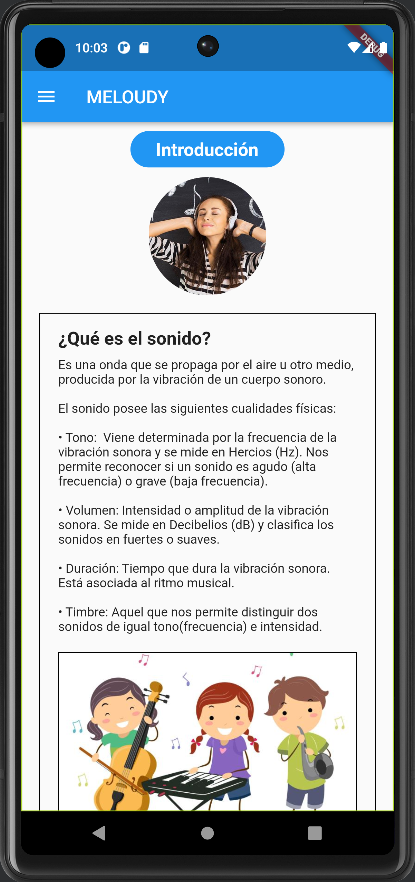
\includegraphics[width=0.44\textwidth]{imagenes/c7/leccion.png} }}%
  \qquad
  \subfloat[\centering Parte 2.]{{ 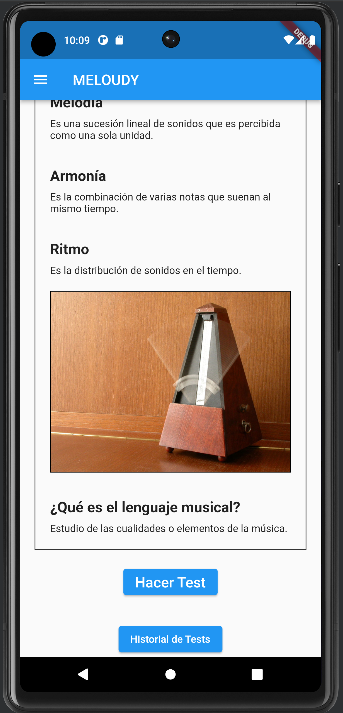
\includegraphics[width=0.44\textwidth]{imagenes/c7/leccion2.png} }}%
  \caption{Pantalla de una lección en concreto con los contenidos (títulos, texto, multimedia...) del temario.}%
  \label{fig:example}%
\end{figure}

\subsection{Test}
\label{sec:test}
La lección contiene un test que se puede realizar al final de la lección. Este test consta de una serie de preguntas que el usuario deberá responder.

\subsubsection{Responder pregunta}
\label{sec:pregunta}
El usuario podrá responder a las preguntas de la siguiente forma: seleccionando una opción de la lista de opciones, seleccionando varias, escribiendo una respuesta en un campo de texto... El usuario podrá 
responder la opción que desee y pasar a la siguiente pregunta. En las siguientes imagenes se pueden ver las pantallas de las distintas preguntas al contestarlas:

\paragraph*{Pregunta de selección única}\mbox{}\\

\label{sec:pregunic1}
\textit{Desarrollado en el Sprint 6}

A continuación se muestra la pantalla de una pregunta de selección única, en la que el usuario deberá seleccionar una opción de la lista de opciones:

\begin{figure}[H]%
  \centering
  \subfloat[\centering Selección única sin una respuesta seleccionada.]{{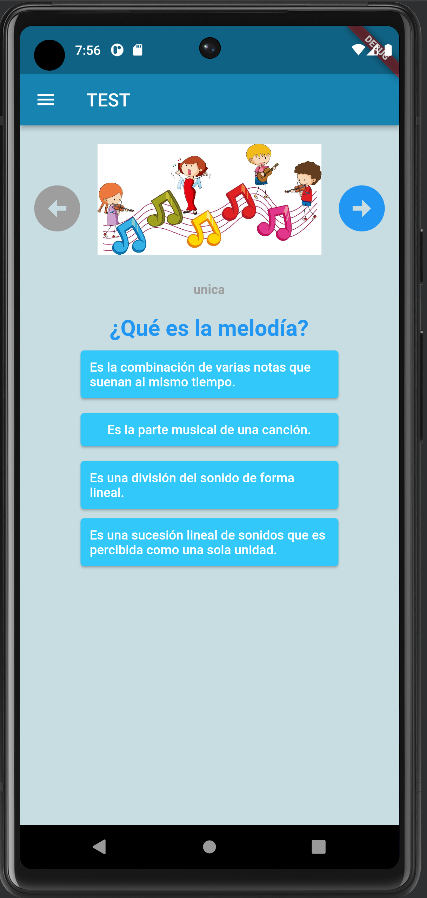
\includegraphics[width=0.45\textwidth]{imagenes/c7/selecunica.png} }}%
  \qquad
  \subfloat[\centering Selección única con una respuesta seleccionada.]{{ 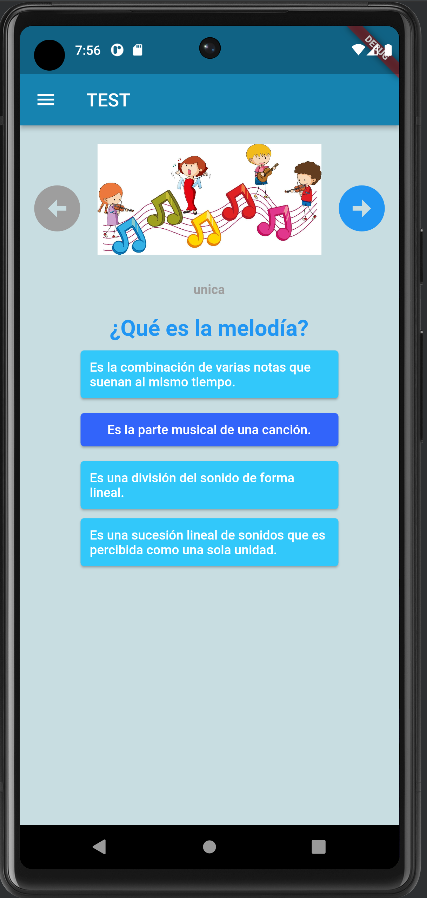
\includegraphics[width=0.45\textwidth]{imagenes/c7/selecunica2.png} }}%
  \caption{Pantalla de una pregunta de selección única en la que las opciones se muestran en forma de lista.}%
  \label{fig:example}%
\end{figure}

\newpage

\paragraph*{Pregunta de selección múltiple}\mbox{}\\

\label{sec:pregunic1}
\textit{Desarrollado en el Sprint 6}

A continuación se muestra la pantalla de una pregunta de selección múltiple, en la que el usuario deberá seleccionar una o varias opciones de la lista de opciones:

\begin{figure}[H]%
  \centering
  \subfloat[\centering Selección múltiple sin una respuesta seleccionada.]{{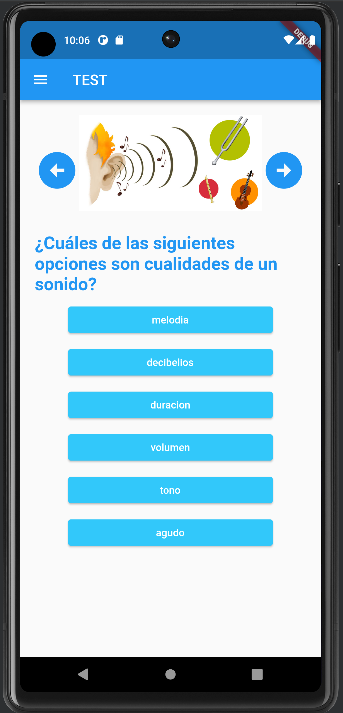
\includegraphics[width=0.45\textwidth]{imagenes/c7/selecmulti.png} }}%
  \qquad
  \subfloat[\centering Selección múltiple con varias respuestas seleccionadas.]{{ 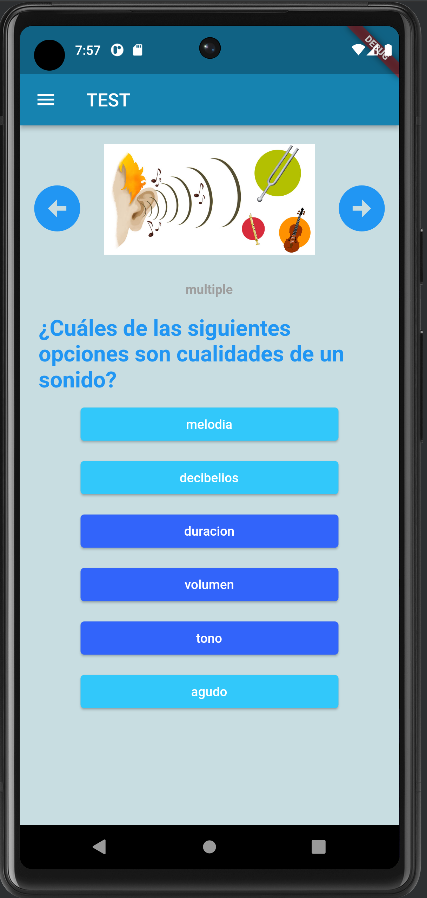
\includegraphics[width=0.45\textwidth]{imagenes/c7/selecmulti2.png} }}%
  \caption{Pantalla de una pregunta de selección múltiple en la que las opciones se muestran en forma de lista.}%
  \label{fig:example}%
\end{figure}



\newpage

\paragraph*{Pregunta de entrada de texto}\mbox{}\\

\label{sec:pregunic1}
\textit{Desarrollado en el Sprint 6}

A continuación se muestra la pantalla de una pregunta de entrada de texto, en la que el usuario deberá escribir la respuesta en un campo de texto:

\begin{figure}[H]%
  \centering
  \subfloat[\centering Entrada de texto sin respuesta introducida.]{{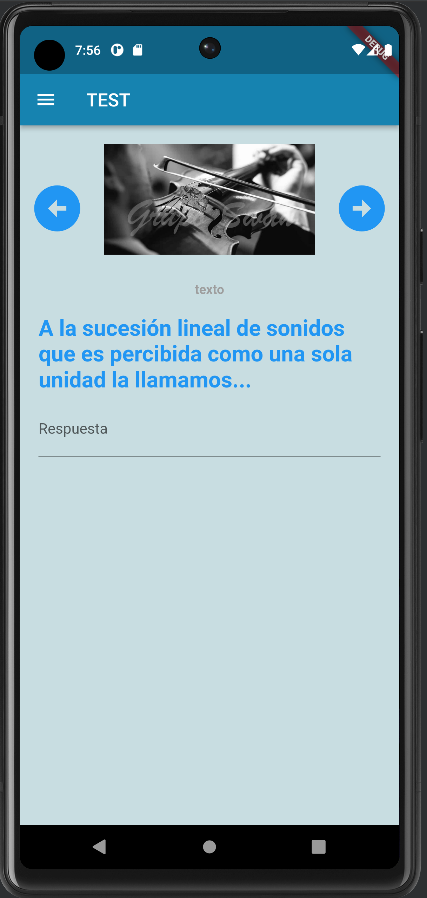
\includegraphics[width=0.45\textwidth]{imagenes/c7/entradatexto.png} }}%
  \qquad
  \subfloat[\centering Entrada de texto con respuesta introducida.]{{ 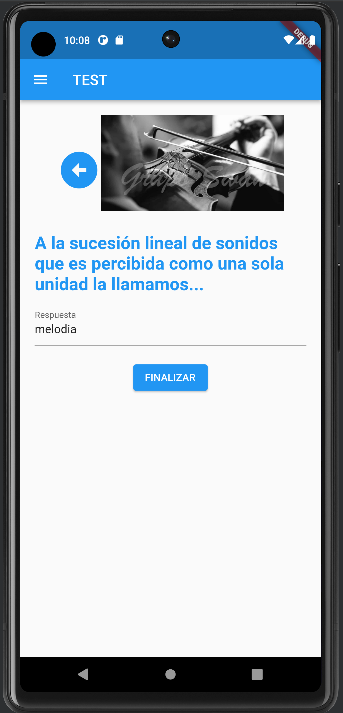
\includegraphics[width=0.45\textwidth]{imagenes/c7/entradatexto2.png} }}%
  \caption{Pantalla de una pregunta de entrada de texto. }%
  \label{fig:example}%
\end{figure}

\newpage

\subsubsection{Resultado del test}\mbox{}\\
\begin{figure}[H]%
  \centering
  \subfloat[\centering Resultado aprobado (50\% o más).]{{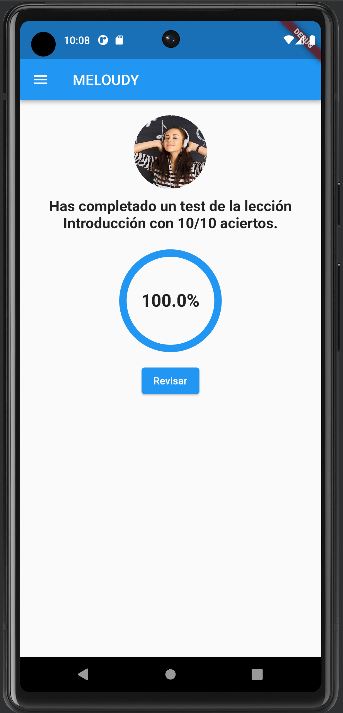
\includegraphics[width=0.45\textwidth]{imagenes/c7/porcentaje.png} }}%
  \qquad
  \subfloat[\centering Resultado suspenso (menos del 50\%).]{{ 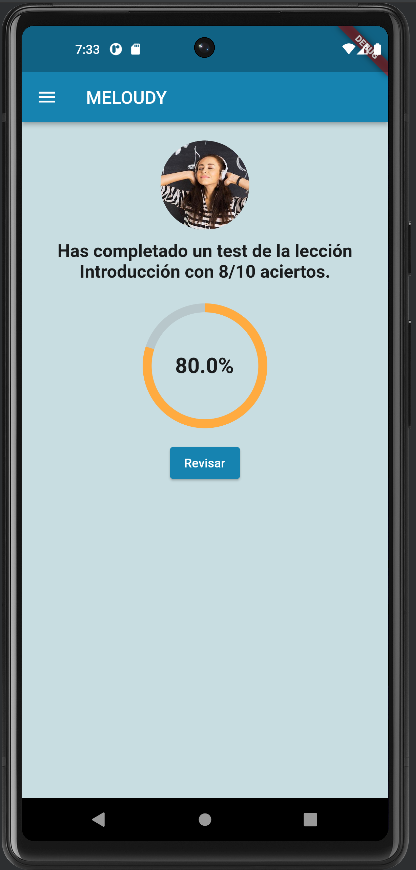
\includegraphics[width=0.45\textwidth]{imagenes/c7/porcentaje2.png} }}%
  \caption{Pantalla que muestra el resultado del test con el número de aciertos y el porcentaje de aciertos respecto a las preguntas con un Progress Bar.}%
  \label{fig:example}%
\end{figure}

\subsubsection{Revisar pregunta}
\label{sec:pregunta}
El usuario podrá revisar las preguntas que haya contestado en un test. Como se puede ver en la pantalla anterior del resultado del test, existe un botón para poder revisar el test. El usuario podrá ver las preguntas que haya contestado y las respuestas que haya seleccionado con la validación de estas.

\paragraph*{Pregunta de selección única}\mbox{}\\
\label{sec:pregunic1b}
\textit{Desarrollado en el Sprint 6}

\begin{figure}[H]%
  \centering
  \subfloat[\centering Selección única acertada.]{{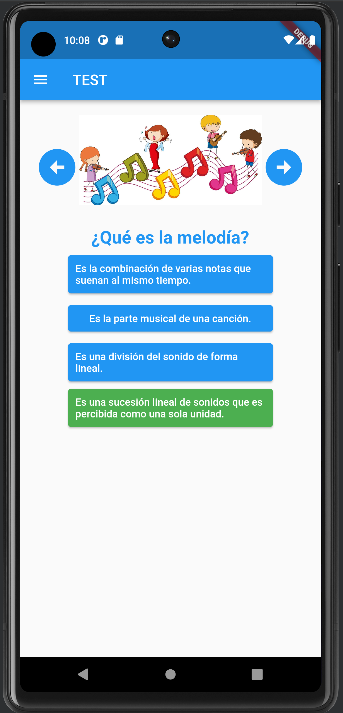
\includegraphics[width=0.45\textwidth]{imagenes/c7/selecunicab.png} }}%
  \qquad
  \subfloat[\centering Selección única fallida.]{{ 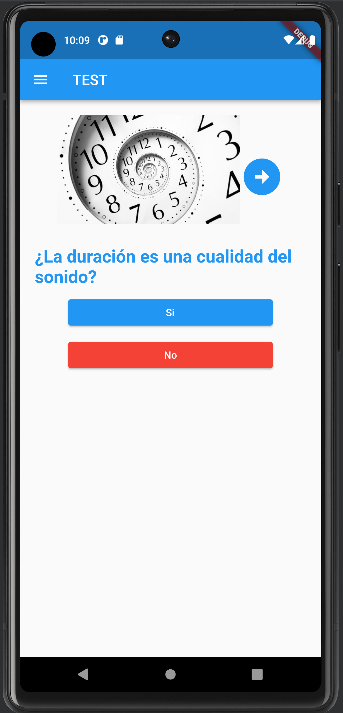
\includegraphics[width=0.45\textwidth]{imagenes/c7/selecunicab2.png} }}%
  \caption{Pantalla de la pregunta de selección única en revisión.}%
  \label{fig:example}%
\end{figure}

\newpage

\paragraph*{Pregunta de selección múltiple}\mbox{}\\
\label{sec:pregunic1b}
\textit{Desarrollado en el Sprint 6}

\begin{figure}[H]%
  \centering
  \subfloat[\centering Selección múltiple acertada.]{{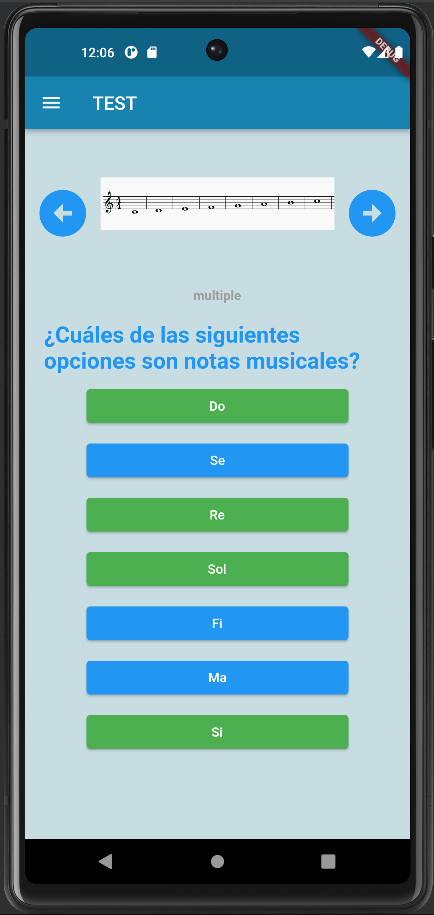
\includegraphics[width=0.45\textwidth]{imagenes/c7/selecmultib.png} }}%
  \qquad
  \subfloat[\centering Selección múltiple fallida.]{{ 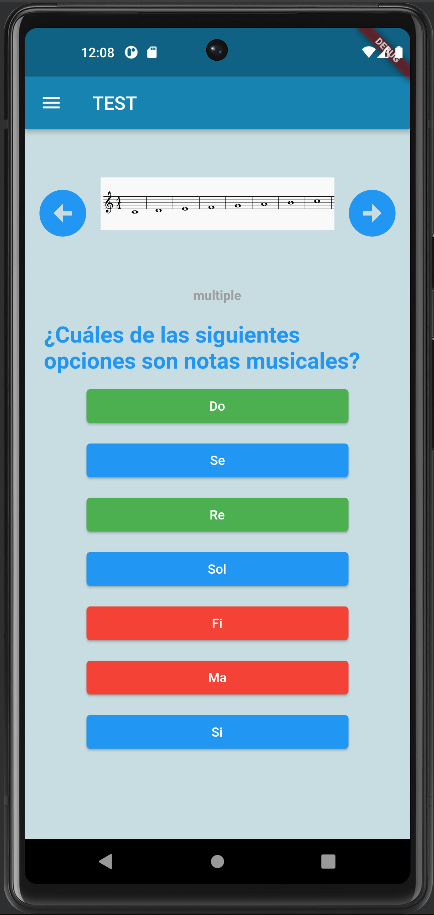
\includegraphics[width=0.45\textwidth]{imagenes/c7/selecmultib2.png} }}%
  \caption{Pantalla de la pregunta de selección múltiple en revisión.}%
  \label{fig:example}%
\end{figure}

\newpage

\paragraph*{Pregunta de entrada de texto}\mbox{}\\

\label{sec:pregunic1b}
\textit{Desarrollado en el Sprint 6}
\begin{figure}[H]%
  \centering
  \subfloat[\centering Entrada de texto acertada.]{{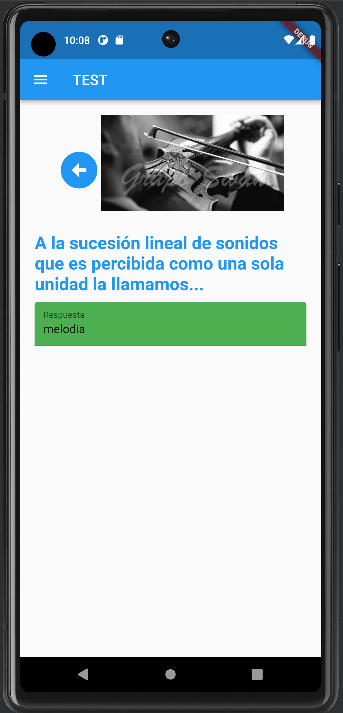
\includegraphics[width=0.45\textwidth]{imagenes/c7/entradatextob.png} }}%
  \qquad
  \subfloat[\centering Entrada de texto fallida.]{{ 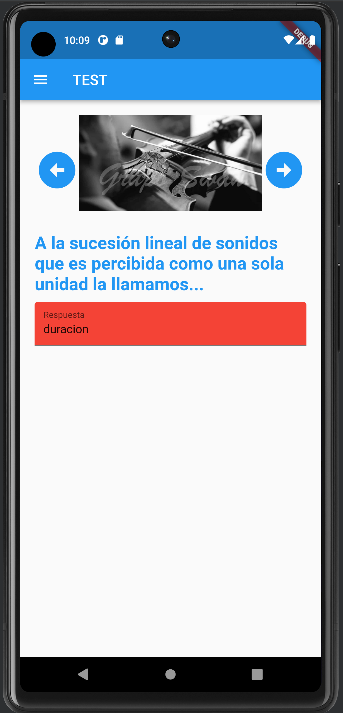
\includegraphics[width=0.45\textwidth]{imagenes/c7/entradatextb2.png} }}%
  \caption{Pantalla de la pregunta de entrada de texto en revisión.}%
  \label{fig:example}%
\end{figure}

\newpage






\section{Funcionalidad del profesor}

\subsection{Dashboard}
\textit{Desarrollado en el Sprint 5}
\label{sec:dashboard}

Un dashboard es una interfaz de usuario que muestra información de forma resumida y que permite al usuario acceder a las diferentes funcionalidades de la aplicación. En este caso, el dashboard del profesor muestra las opciones de gestión de lecciones y preguntas.

\paragraph*{Vista}
Se ha implementado una pantalla de dashboard para la gestión de la aplicación. En esta pantalla, se muestran las opciones de gestión disponibles para la persona que utiliza la aplicación en función de su rol mediante una columna de ElevatedButton. En la siguiente imagen se puede ver la pantalla de dashboard:

\begin{figure}[H]
  \centering
  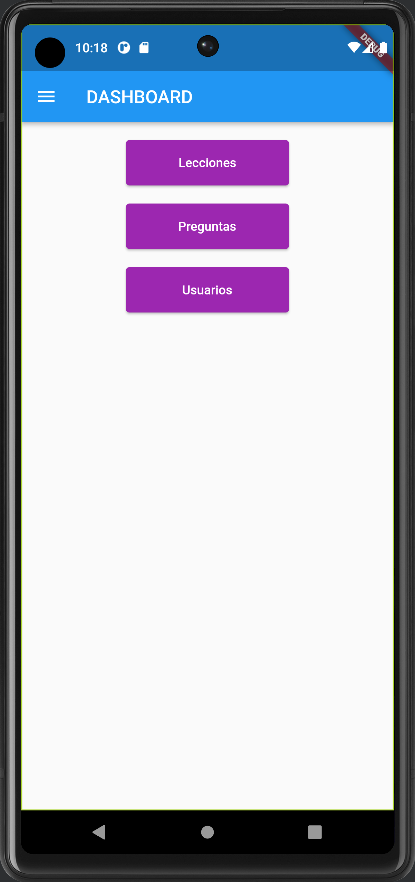
\includegraphics[width=0.4\textwidth]{imagenes/c7/dashboard.png}
  \caption{Pantalla de dashboard}
  \label{fig:login}
\end{figure}


\subsection{Lista de lecciones} 
\textit{Desarrollado en el Sprint 5}

\paragraph*{Vista}
La lista de lecciones del profesor es muy similar a la del usuario. Las diferencias, aparte de los estilos, son los botones de tipo ElevatedButton que se han añadido para la gestión de las lecciones y que permiten al profesor crear y eliminar lecciones. En la siguiente imagen se puede ver la pantalla de lista de lecciones del profesor:

\begin{figure}[H]
  \centering
  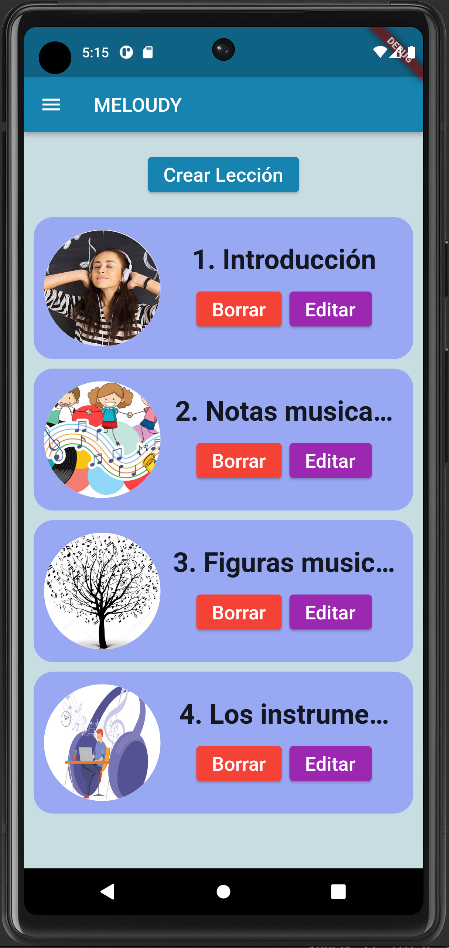
\includegraphics[width=0.4\textwidth]{imagenes/c7/listalecciones.png}
  \caption{Pantalla de inicio de sesión}
  \label{fig:login}
\end{figure}